\documentclass[a4paper,12pt]{article}
\usepackage{amsmath, amssymb, amsfonts}
\usepackage[utf8]{inputenc}
\usepackage[russian]{babel}
\usepackage{geometry}
\geometry{top=2cm, bottom=2cm, left=2.5cm, right=2.5cm}
\usepackage{enumitem}
\usepackage{hyperref}
\usepackage{graphicx}
\usepackage{tikz}             % Пакет для рисования
\usetikzlibrary{arrows.meta}
\usetikzlibrary{calc}  % Библиотека для более гибких стрелок (опционально)


\begin{document}

\begin{center}
    \textbf{2024}\\
    \textbf{ТФКП, семестр 3. Преподаватель: Вакаева А.Б.}\\
    \vspace{1cm}
    \textbf{Вариант 6}\\
    \textbf{Группа 23.Б16-пу}
\end{center}

\vspace{1cm}

1. Написать всевозможные разложения по степеням $z - z_0$:
\begin{equation*}
    \frac{5z}{(z+2)(z-3)}.
\end{equation*}

Необходимые темы:
\begin{itemize}
    \item \href{https://ru.wikipedia.org/wiki/Ряд_Тейлора}{Разложение функций в ряд Тейлора}
    \item \href{https://ru.wikipedia.org/wiki/Ряд_Лорана}{Ряды Лорана}
    \item \href{https://ru.wikipedia.org/wiki/Дробно-рациональная_функция}{Декомпозиция 
    дробно-рациональных функций}
    \item \href{https://ru.wikipedia.org/wiki/Область_сходимости}{Определение области 
    сходимости ряда}
\end{itemize}

\vspace{0.5cm}

2. Найти все особые точки, определить их характер, найти вычеты в изолированных 
особых точках, включая бесконечно удаленную точку:
\begin{equation*}
    f(z) = e^{\frac{z^2+1}{z}}.
\end{equation*}

Необходимые темы:
\begin{itemize}
    \item \href{https://ru.wikipedia.org/wiki/Особая_точка}{Особые точки в комплексном 
    анализе}
    \item \href{https://ru.wikipedia.org/wiki/Классификация_особых_точек}{Классификация 
    особых точек (полюса, устранимые, существенные)}
    \item \href{https://ru.wikipedia.org/wiki/Ряд_Лорана}{Разложение в ряд Лорана для 
    нахождения вычетов}
    \item \href{https://ru.wikipedia.org/wiki/Вычет}{Теорема о вычетах и вычисление 
    вычетов}
    \item \href{https://ru.wikipedia.org/wiki/Бесконечно_удаленная_точка}{Особенности 
    бесконечно удаленной точки}
\end{itemize}

\vspace{0.5cm}

3. Вычислить:
\begin{equation*}
    \int\limits_0^{2\pi} \frac{\sin^2 x \, dx}{a + b \cos x}, \quad a > b > 0.
\end{equation*}

Необходимые темы:
\begin{itemize}
    \item \href{https://ru.wikipedia.org/wiki/Тригонометрические_интегралы}{Тригонометрические 
    интегралы}
    \item \href{https://ru.wikipedia.org/wiki/Комплексный_анализ}{Применение комплексного 
    анализа в вычислении интегралов}
    \item \href{https://ru.wikipedia.org/wiki/Теорема_о_вычетах}{Метод вычетов для 
    вычисления интегралов}
    \item \href{https://ru.wikipedia.org/wiki/Замена_переменных}{Метод замены переменных 
    в интегралах}
\end{itemize}

\newpage
\section{Теория по задачам}
\subsection{1 задача}
\textbf{Многочлен} Тейлора: (в случае если функция бесконечно диф-ма в окрестности
    этой точки, то тогда это \textbf{Ряд} Тейлора, иными словами это Разложение
    функции по положительным степеням в ряд Тейлора)
\begin{figure}[h]     
    \centering     
    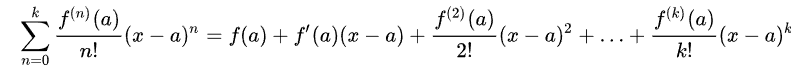
\includegraphics[width=0.8\textwidth]{2025-02-24-19-33-49.png}     
    \caption{Caption for }     
    \label{} 
\end{figure}

При $a = 0$ такой ряд называнется - рядом Маклорена

Рядом Тейлора в точке $a$ функции $f(z)$ комплекной переменной $z$, удовлетворяющей в 
    некоторой окрестности $U \subseteq \mathbb{C}$ условаиям Коши-Риммана, называется
    степенной ряд
\begin{figure}[h]     
    \centering     
    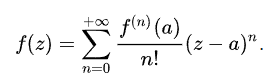
\includegraphics[width=0.8\textwidth]{2025-02-24-19-50-22.png}     
    \caption{Caption for }     
    \label{} 
\end{figure}

Условия Коши-Риммана в Комплексной плоскости (Эйлера-Доламбера) - это соотношения 
связываемые веществую часть $u = u(x,y)$ и мнимую часть $v = v(x,y)$ всякой функции 
комплексного переменного $w = f(z) = u + iv, \ z = x + iy$

\begin{figure}[h]     
    \centering     
    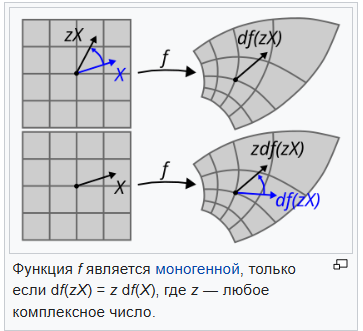
\includegraphics[width=0.5\textwidth]{2025-02-24-20-41-56.png}     
    \caption{Caption for }     
    \label{} 
\end{figure}

Требование, что $df$ пропорционально $dz$ одним и тем же комплексным числом
 независимо от направления приращения $dz$, называется \textbf{условиями Коши-Римана}.

Условия Коши-Риммана:
\begin{equation*}
    \frac{\partial u}{\partial x} = \frac{\partial v}{\partial y}, \quad \frac{\partial 
    u}{\partial y} = -\frac{\partial v}{\partial x}
\end{equation*}

\subsection{Конформность}
Функция $f(z)$ называется конформной, если она сохраняет углы между пересекающимися 
кривыми. Это означает, что функция $f(z)$ сохраняет форму малых фигур при отображении.

\subsection{Смысл условий Коши-Римана}
Условия Коши-Римана являются необходимыми и достаточными условиями для того, чтобы 
функция комплексного переменного $f(z)$ была аналитической. Они обеспечивают, что 
функция $f(z)$ дифференцируема в комплексном смысле и, следовательно, конформна. Эти 
условия связывают частные производные вещественной и мнимой частей функции, обеспечивая 
согласованность их изменений.

\begin{tikzpicture}[scale=1.5, >=stealth] 
    % Рисуем оси
    \draw[->] (-0.5,0) -- (3.5,0) node[anchor=north] {$\Re(z)$};
    \draw[->] (0,-0.5) -- (0,3.5) node[anchor=east] {$\Im(z)$};

    % Координаты точки z0
    \coordinate (Z0) at (1.5,1.5);

    % Ставим точку z0 и подписываем
    \fill (Z0) circle (1.5pt) node[anchor=north east] {$z_0$};

    % Координаты точки (z0 + Delta z) - например, сдвигаем на (0.8,1)
    \coordinate (Z1) at ($(Z0)+(0.8,1)$);

    % Рисуем сам вектор Delta z (от z0 до z0+Delta z)
    \draw[->, thick, blue] (Z0) -- (Z1) node[midway, anchor=south west] {$\Delta z$};

    % (Опционально) штриховые линии от начала координат для наглядности
    \draw[dashed] (0,0) -- (Z0);
    \draw[dashed] (0,0) -- (Z1);
\end{tikzpicture}

\subsection{Различия комплексной дифференцируемости и дифференцируемости вещественной
    функции}
Суть в том, что вещественная функция дифференцируема в точке, если ее приращение
можно представить в виде суммы приращения функции и линейного приращения. В случае
комплексной функции, дифференцируемость означает, что приращение функции можно
представить в виде суммы приращения функции и линейного приращения, умноженного на
комплексное число.

Формула дифференциала для комплексных чисел:
\begin{equation*}
    df = \frac{\partial u}{\partial x} dx + \frac{\partial u}{\partial y} dy + 
    i\left(\frac{\partial v}{\partial x} dx + \frac{\partial v}{\partial y} dy\right)
\end{equation*}

ЗАмечание: в комплексном дифференцировании нам не важно знать направление функции,
функция может стремиться в точку с любого направления, т.к. это \(\mathbf{R}^2\) 
пространство в переводе на вещественное пространство.

\subsection{Ряд Лорана}
\textbf{Ряд Лорана} - это разложение функции в ряд, содержащий как положительные, так и
отрицательные степени переменной. Ряд Лорана является обобщением ряда Тейлора.

Формула ряда Лорана:
\begin{equation*}
    f(z) = \sum_{n=-\infty}^{\infty} c_n (z - z_0)^n,
\end{equation*}
где коэффициенты $c_n$ определяются как:
\begin{equation*}
    c_n = \frac{1}{2\pi i} \int_{\gamma} \frac{f(\zeta)}{(\zeta - z_0)^{n+1}} \, d\zeta,
\end{equation*}
и $\gamma$ - замкнутый контур, охватывающий точку $z_0$. Ряд Лорана сходится в кольце
$R = \{z: r < |z - z_0| < R\}$, где $r$ - радиус сходимости ряда Тейлора, а $R$ - радиус
сходимости ряда Лорана.


\subsection{Теорема Лорана}

Применение рядов Лорана основано главным образом на следующей теореме Лорана:

\textbf{Теорема Лорана.}
Пусть функция $f(z)$ аналитическая (однозначная) в кольце
\[
A = \{\,z : r < |z - z_0| < R \}.
\]
Тогда она представима в этом кольце \textit{разложением в ряд Лорана} по степеням $(z - z_0)$, сходящимся во всём кольце $A$:
\[
f(z) \;=\; \sum_{n=-\infty}^{+\infty} a_n \,(z - z_0)^n.
\]
Данное разложение служит основой для исследования поведения функции $f(z)$ в окрестности точки $z_0$, если эта точка является \textit{особой} (не принадлежит области аналитичности функции).

\vspace{2ex}
В зависимости от типа особой точки $z_0$ различают:
\begin{itemize}
    \item \textbf{Устранимая особая точка} (если часть ряда Лорана с отрицательными степенями отсутствует или может быть сведена к нулю).
    \item \textbf{Полюс} (если в ряде Лорана содержится конечное число членов с отрицательными степенями).
    \item \textbf{Существенная особая точка} (если в ряде Лорана бесконечно много членов с отрицательными степенями).
\end{itemize}
\href{https://www.youtube.com/watch?v=BGf3L-MLWc8&list=PL_RWQIyLkfYulHxhBfXHhFxmqouU3U2Jd&index=32}{Разложение на всевозможные степени}

\subsection{Особые точки: исторические названия и их смысл}

В комплексном анализе особые точки (или сингулярности) классифицируются на три основных типа:
\textbf{устранимая особая точка}, \textbf{полюс} и \textbf{существенная особая точка}.
Исторически эти названия отражают различные способы, которыми ``ломается'' аналитичность функции в окрестности такой точки.

\subsection{Устранимая особая точка}
Получила название из-за того, что ``сингулярность'' (нарушение аналитичности) можно \textit{устранить} (или \textit{исправить}) путём подходящего определения (или переопределения) значения функции в этой точке. 
Если в ряде Лорана отсутствуют члены с отрицательными степенями, то функцию можно аналитически продолжить на эту точку, и она перестаёт быть особой.

\subsection{Полюс}
Название возникло в связи с тем, что при приближении к точке модуль функции ``возрастает до бесконечности''.
В вещественном анализе аналогом является вертикальная асимптота, напоминающая ``столб'' или ``полюс''. 
В ряде Лорана при полюсе появляется конечное число членов с отрицательными степенями, и поведение функции похоже на
\[
\frac{1}{(z - z_0)^n},
\]
что образно воспринимается как ``столб'', уходящий в бесконечность.

\subsection{Существенная особая точка}
Слово ``существенная'' (или ``основная'', ``важная'') подчеркивает, что такая точка даёт наиболее ``сложное'' поведение функции:
в ряде Лорана возникает бесконечно много отрицательных степеней, и функцию нельзя свести к полюсу или устранить переопределением.
Классический пример --- экспонента \( e^{\tfrac{1}{z}} \) в точке \( z = 0 \), у которой в разложении в ряд Тейлора по \( 1/z \) присутствуют все степени.
Подобная ``существенная'' сингулярность ведёт к сильным и интересным результатам, например, к теореме Пикара:
в окрестности существенной особой точки функция принимает \emph{почти все} возможные комплексные значения.


\end{document}
